% BEGIN PREAMBEL
\documentclass[9pt]{beamer}
\usepackage[british]{babel}
\usepackage[latin1]{inputenc}
\usepackage{multimedia}
\usepackage{amsmath,amsfonts,amssymb}
\usepackage{upgreek}
\usepackage{pgfpages}
\usepackage[version=3]{mhchem}
\usepackage{lmodern}
\usepackage{graphicx}
\usepackage{multicol}
\usepackage{xcolor}
\usepackage{wrapfig}
\newcommand{\as}{\\[14pt]}
\newcommand{\s}{\\[7pt]}
\newcommand{\is}{\\[2pt]}
\newcommand{\no}{\noindent}
\newcommand{\ka}{\hspace*{0.5cm}}
\newcommand{\ma}{\hspace*{1cm}}
\newcommand{\ga}{\hspace*{1.5cm}}
\newcommand{\li}{\left|}
\newcommand{\re}{\right|}
\newcommand{\const}{\text{const.}}
\newcommand{\z}{\text}
\newcommand{\terminal}[1]{\colorbox{black}{\textcolor{white}{{\fontfamily{phv}\selectfont \scriptsize{#1}}}}}
\newcommand{\plugin}[1]{\textit{\flq#1\frq}}
\usetheme{Boadilla}
\graphicspath{ {Pics/} }
\usecolortheme{beaver}
\useoutertheme{miniframes}
\beamertemplatenavigationsymbolsempty
\makeindex
\title[Analysis]{Discussion of the Pad Analysis}
\author[M. Reichmann]{Michael Reichmann}
\institute[\textbf{\textit{ETH}}\scalebox{.6}{\textit{Z\"{u}rich}}]{Swiss Federal Institute of Technology Zurich}
% END PREAMBEL
\begin{document}
% ============================
% TITLE PAGE
% ============================
\begin{frame}
	\begin{center}
		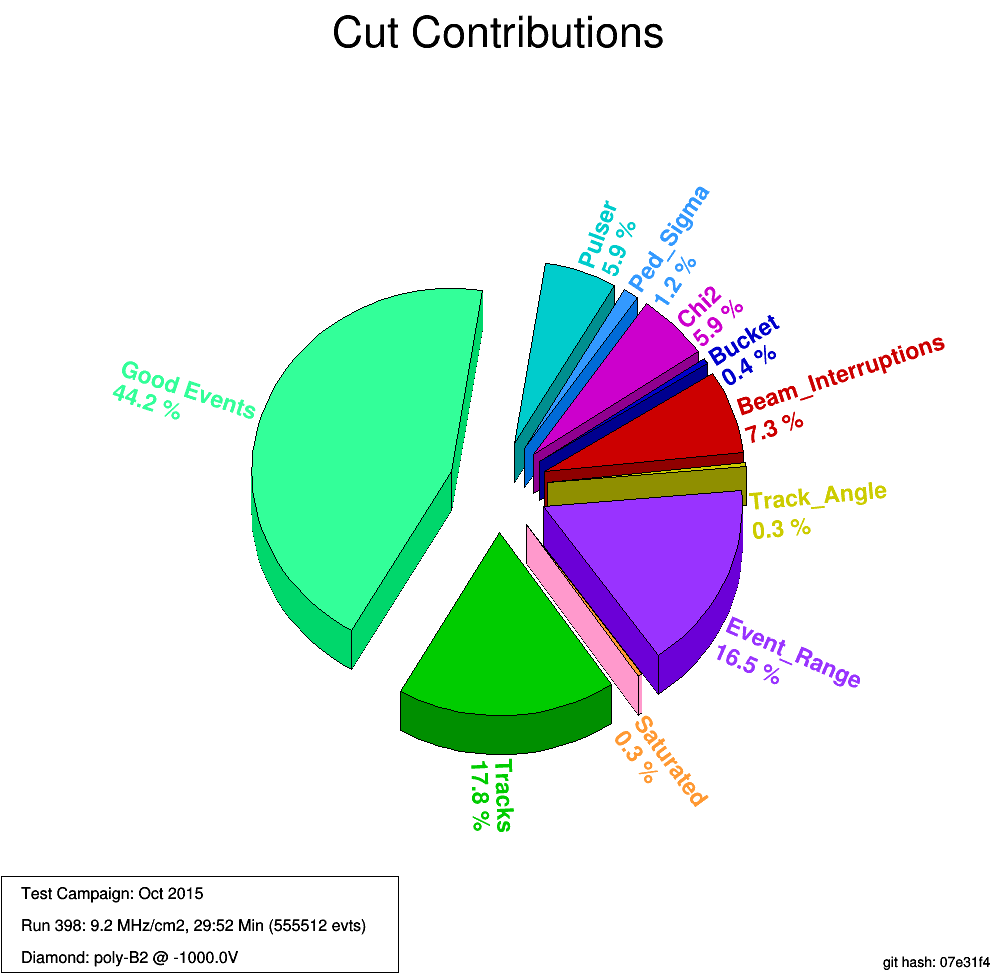
\includegraphics[width=6cm]{CutContributions}
	\end{center}
	\begin{alertblock}{
		\begin{center}
			\textbf{Meeting \today}
		\end{center}}
		\vspace*{10pt}
		\begin{center}\small
		Michael Reichmann
		\end{center}\normalsize
	\end{alertblock}
\end{frame}
% ============================
% TABLE OF CONTENTS
% ============================
\begin{frame}[allowframebreaks]
	\frametitle{Table of contents}
	\tableofcontents   % [pausesections]
\end{frame}
% ====================================================================================
% SLIDES
% ====================================================================================
\section{Beam Profile}
% ============================
\subsection{Profiles}
\begin{frame}
	\begin{center}
		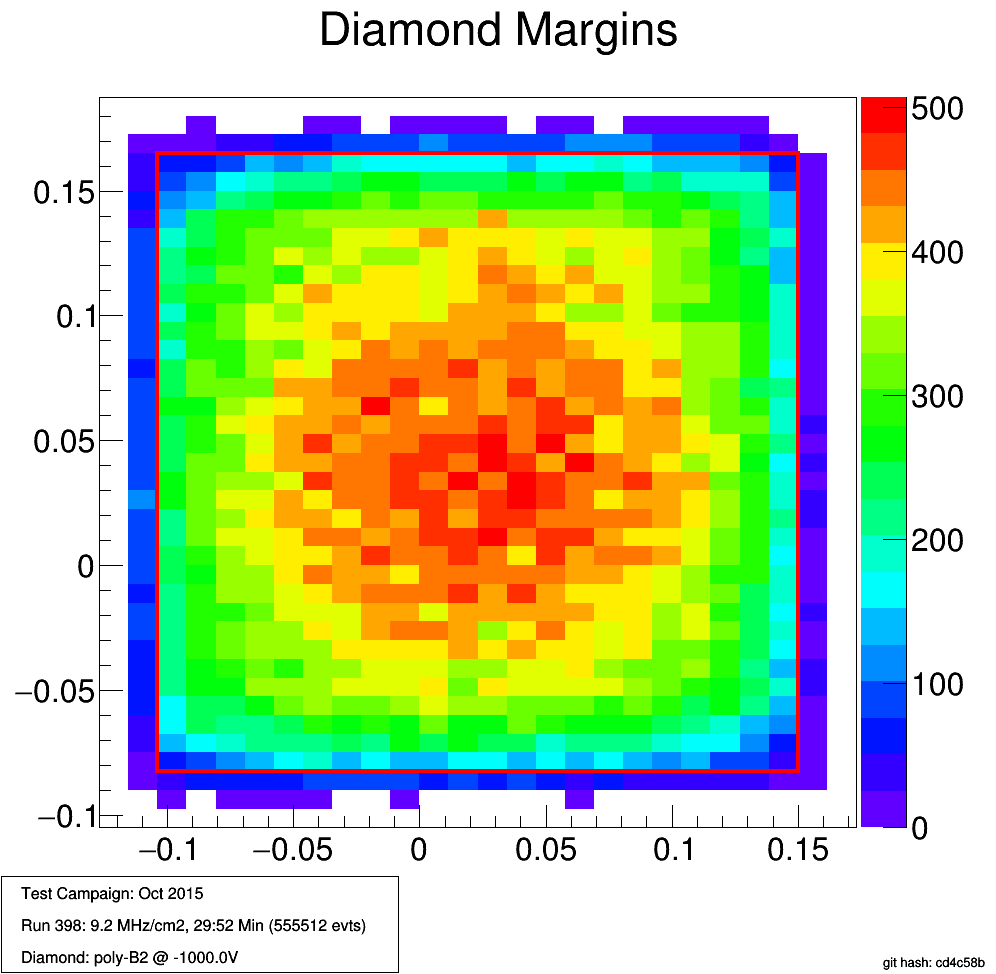
\includegraphics[width=4cm]{DiamondHitmap}
	\end{center}

	\begin{center}
		\begin{minipage}{4cm}
			\centering
			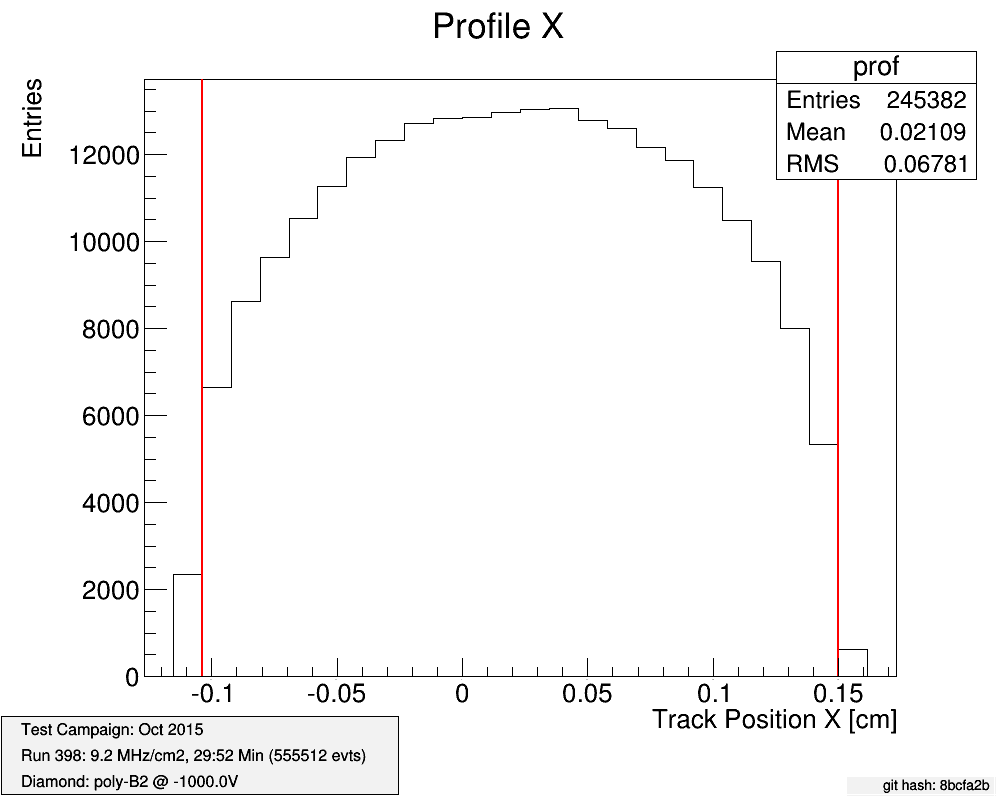
\includegraphics[width=4cm]{BeamProfileX}
		\end{minipage}
		\hspace*{2pt}
		\begin{minipage}{4cm}
			\centering
			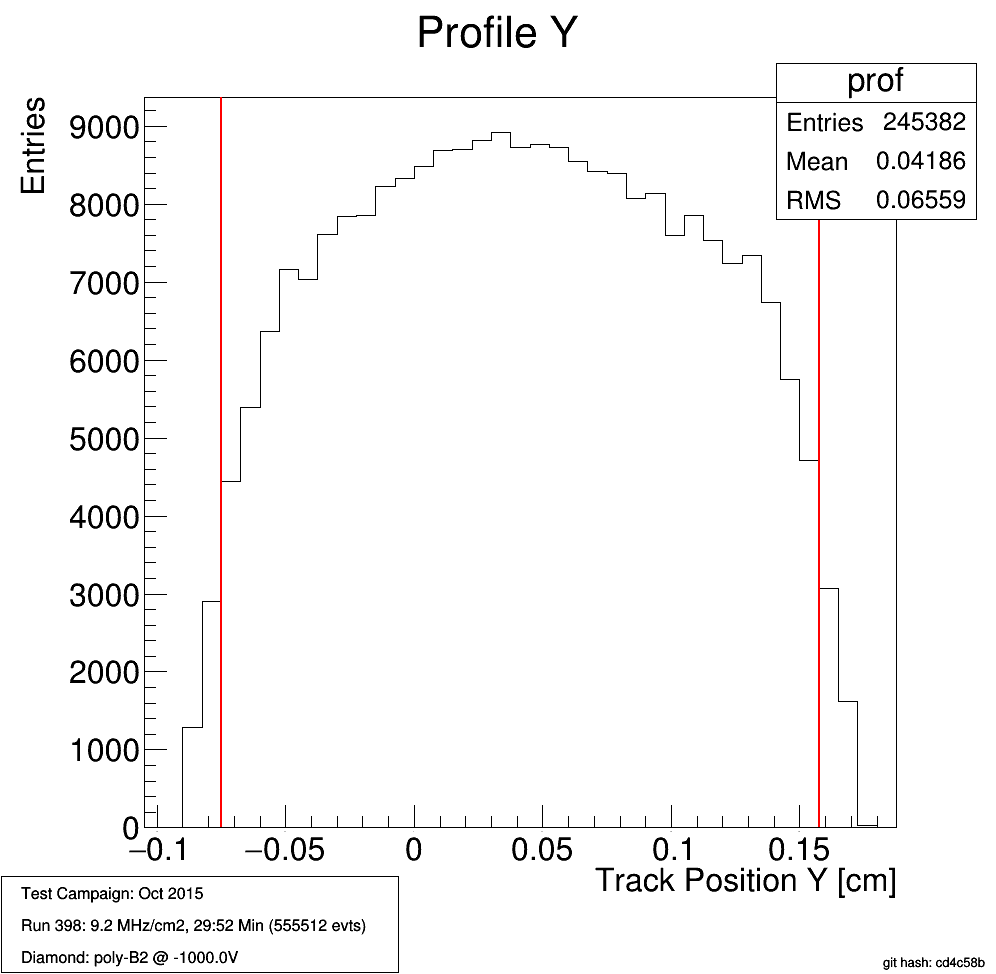
\includegraphics[width=4cm]{BeamProfileY}
		\end{minipage}\no\s
	\end{center}
\end{frame}
% new frame ============================
\begin{frame}
	\begin{center}
		\begin{minipage}{5.5cm}
			\centering
			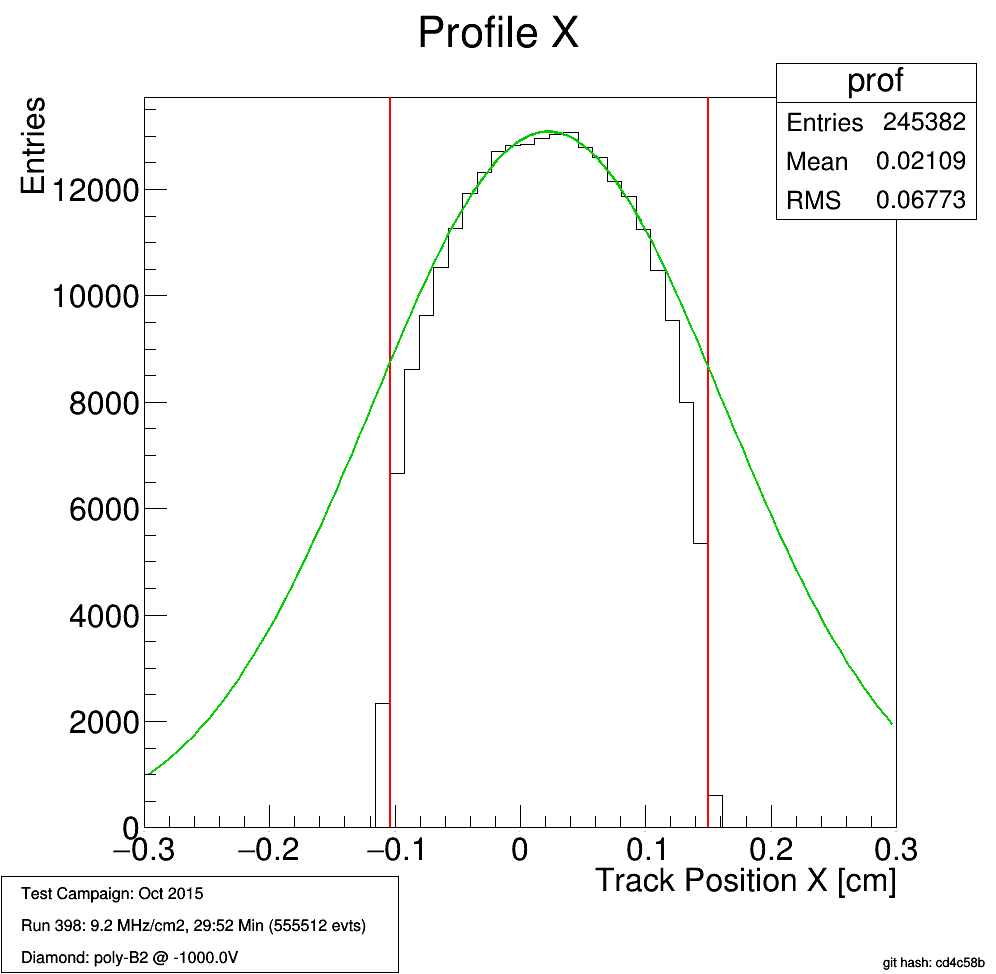
\includegraphics[width=5.5cm]{BeamProfileXFit}
		\end{minipage}
		\hspace*{2pt}
		\begin{minipage}{5.5cm}
			\centering
			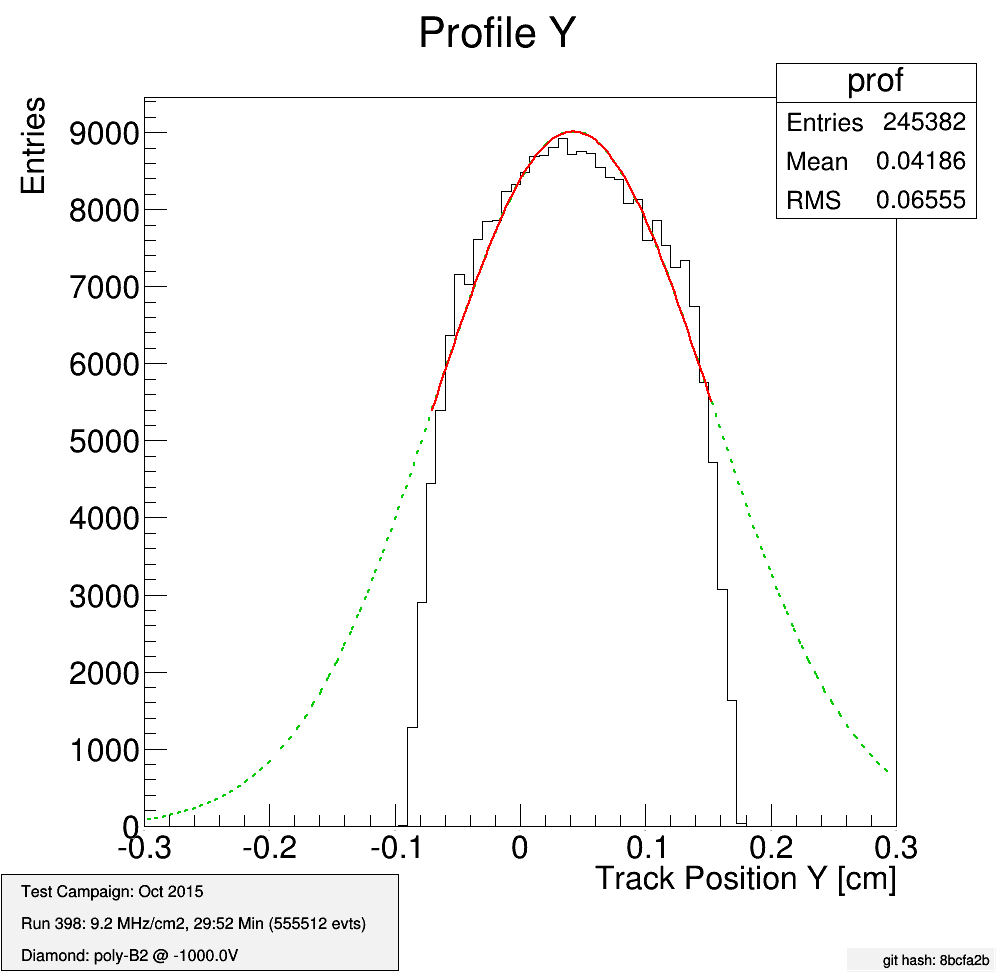
\includegraphics[width=5.5cm]{BeamProfileYFit}
		\end{minipage}\no\s
	\end{center}
	\begin{itemize}
		\item looking for center of the mask ($\approx$ center of red lines)
		\item fit Gauss in which range around this center?? 
		\item plots for 60\% of the the red lines 
	\end{itemize}

\end{frame}
% new frame ============================
\begin{frame}
	\begin{center}
		\begin{minipage}{5.5cm}
			\centering
			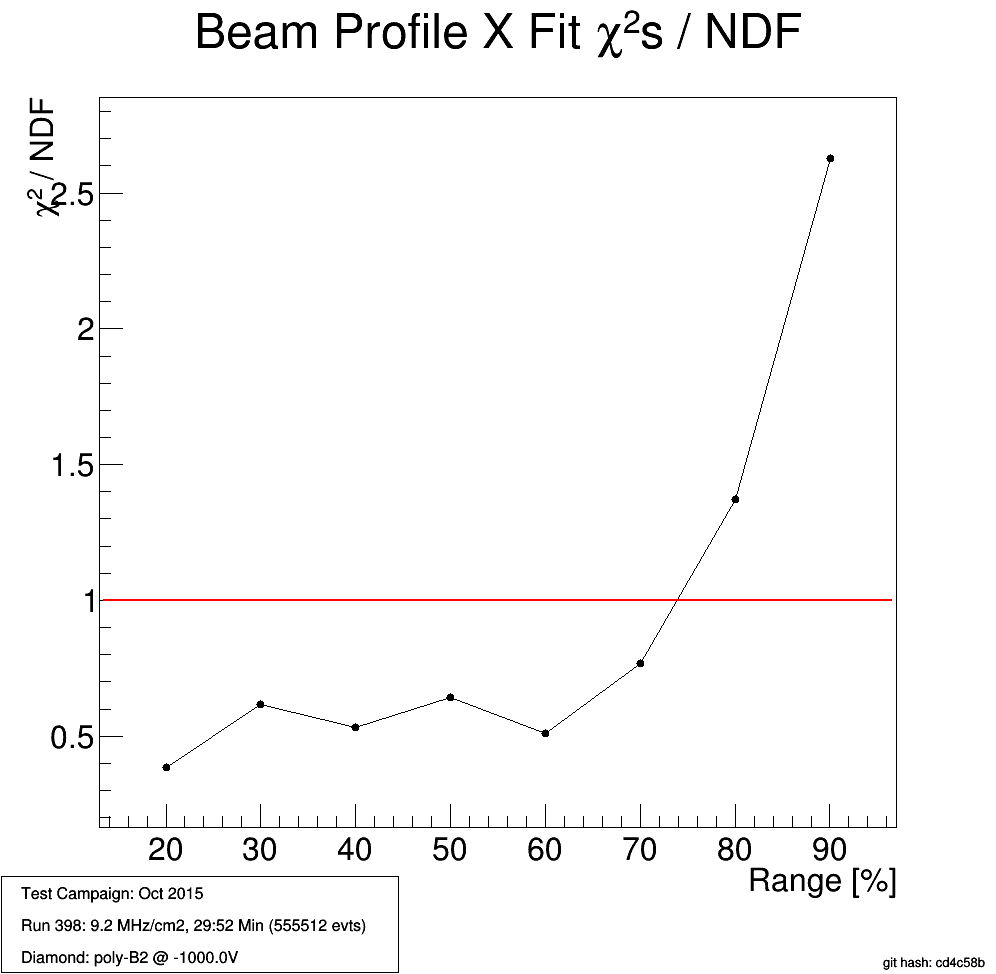
\includegraphics[width=5.5cm]{BeamProfChi2sX}
		\end{minipage}
		\hspace*{2pt}
		\begin{minipage}{5.5cm}
			\centering
			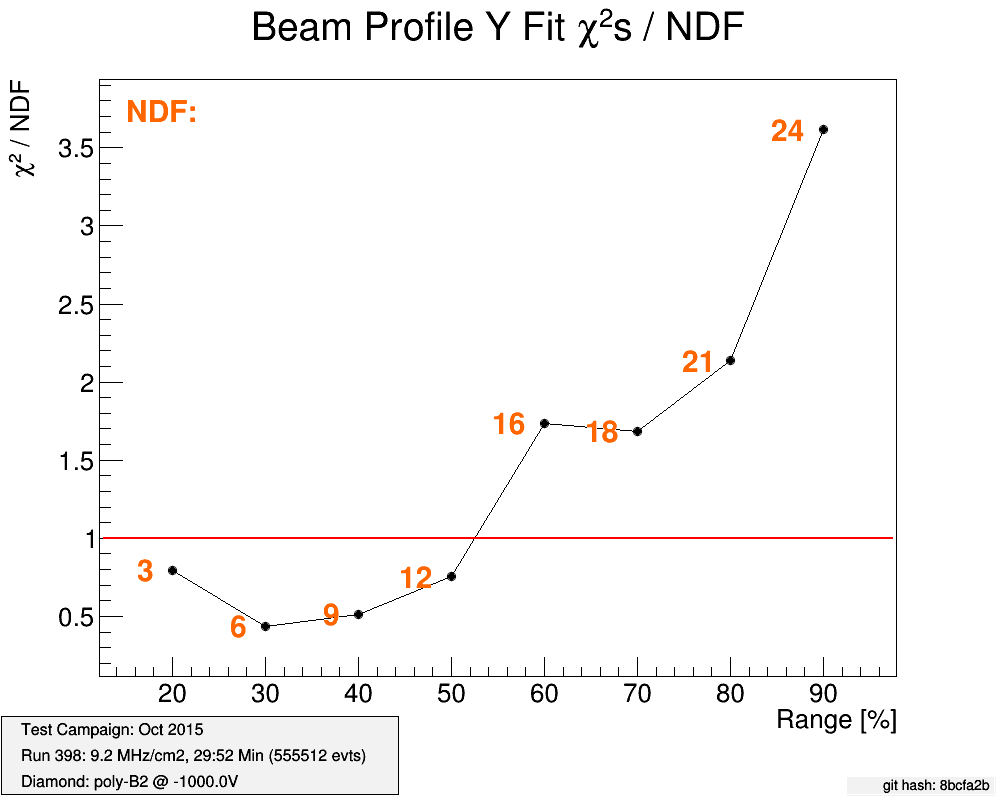
\includegraphics[width=5.5cm]{BeamProfChi2sY}
		\end{minipage}\no\s
	\end{center}
\end{frame}
% new frame ============================
\begin{frame}
	\begin{center}
		\begin{minipage}{5.5cm}
			\centering
			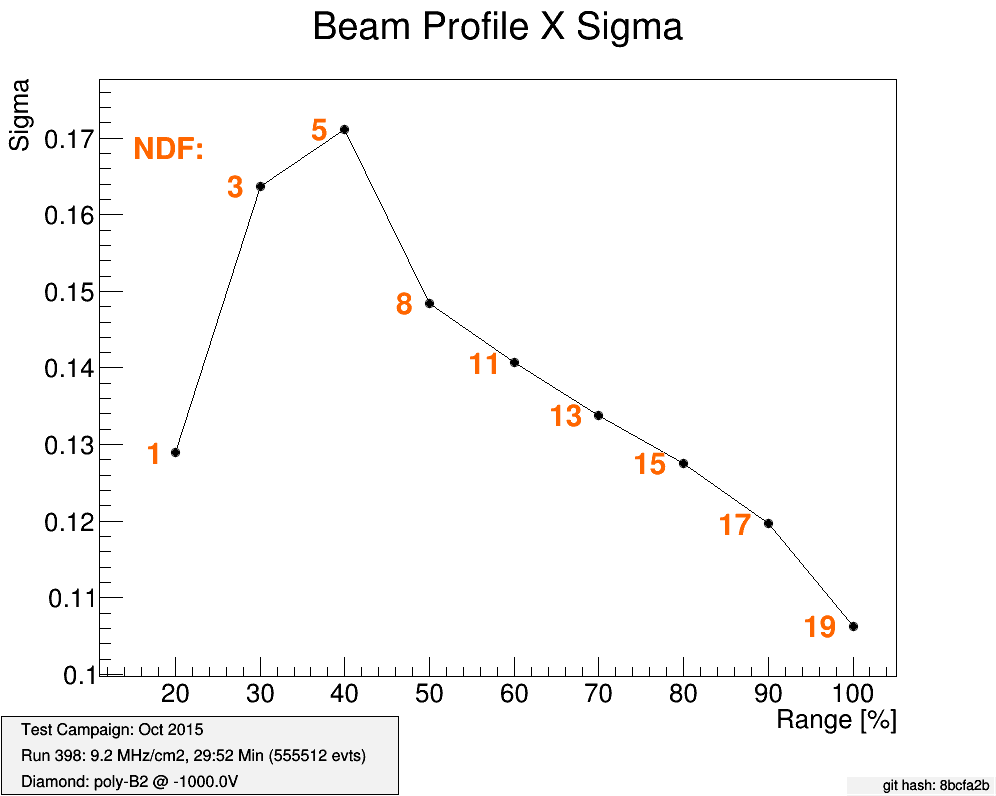
\includegraphics[width=5.5cm]{BeamProfSigmasX}
		\end{minipage}
		\hspace*{2pt}
		\begin{minipage}{5.5cm}
			\centering
			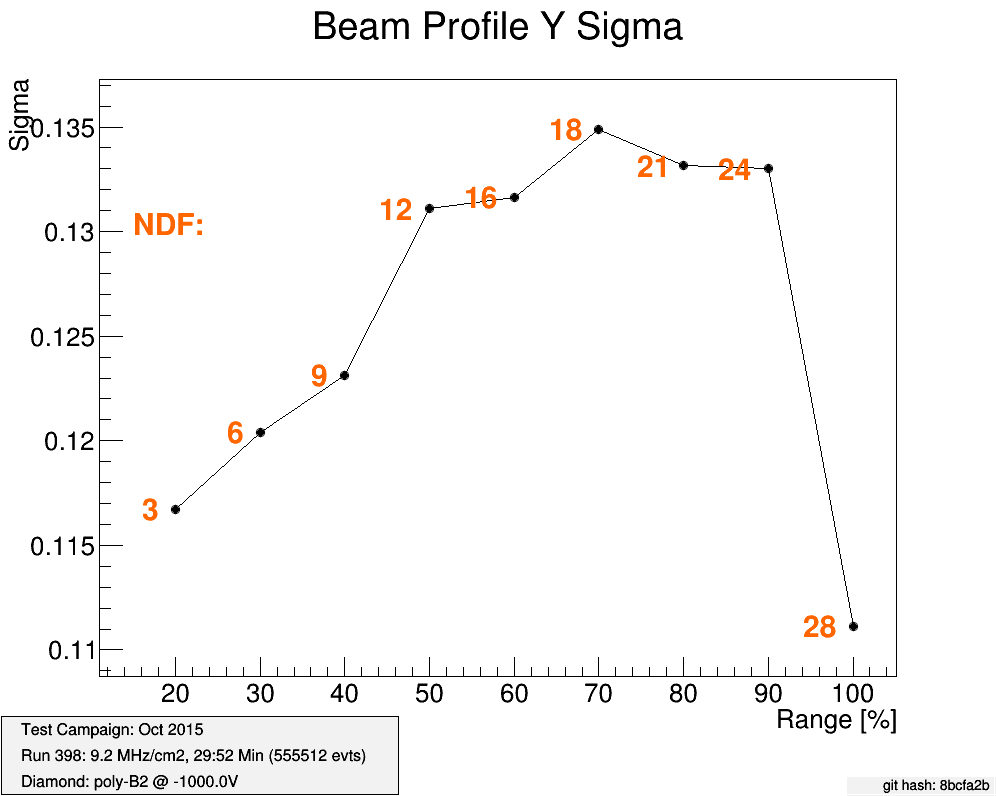
\includegraphics[width=5.5cm]{BeamProfSigmasY}
		\end{minipage}\no\s
	\end{center}
\end{frame}
% new frame ============================
% ============================
\subsection{Rate dependence}
\begin{frame}
	\frametitle{Rate dependence}
	\begin{center}
		\begin{minipage}{5.5cm}
			\centering
			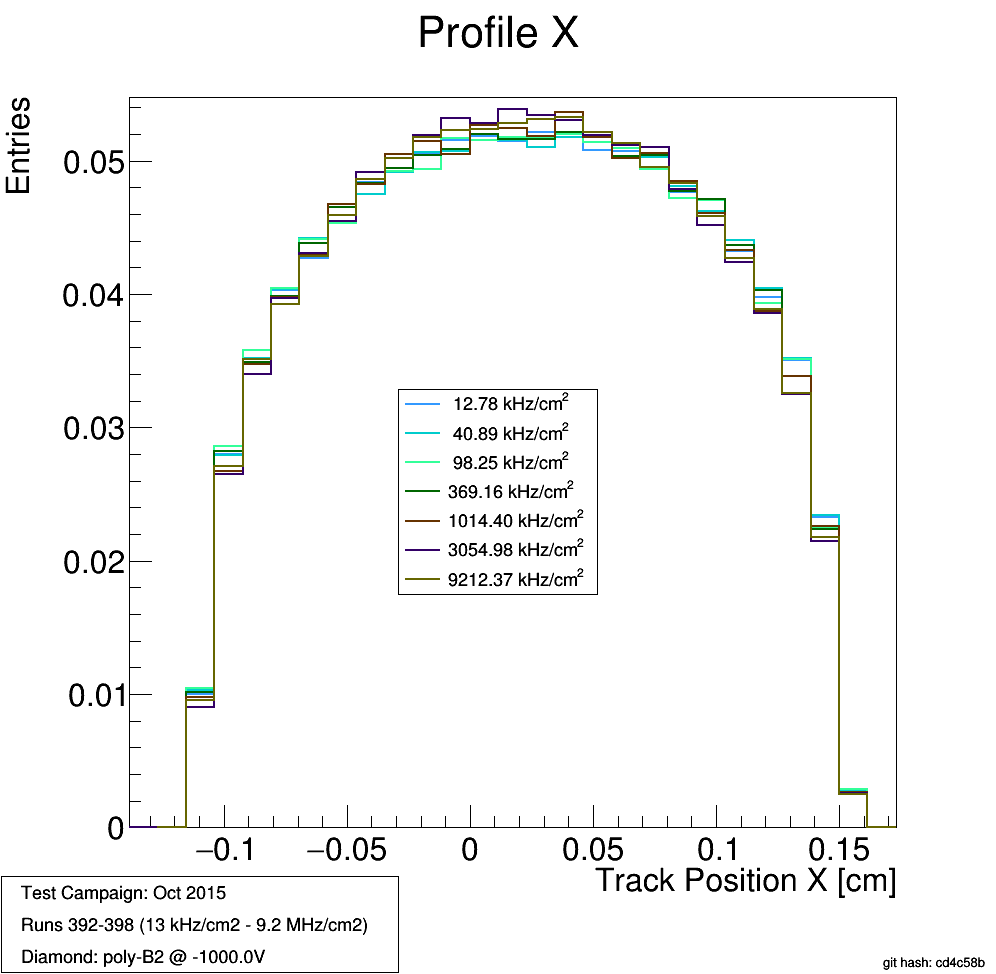
\includegraphics[width=5.5cm]{AllBeamProfilesX}
		\end{minipage}
		\hspace*{2pt}
		\begin{minipage}{5.5cm}
			\centering
			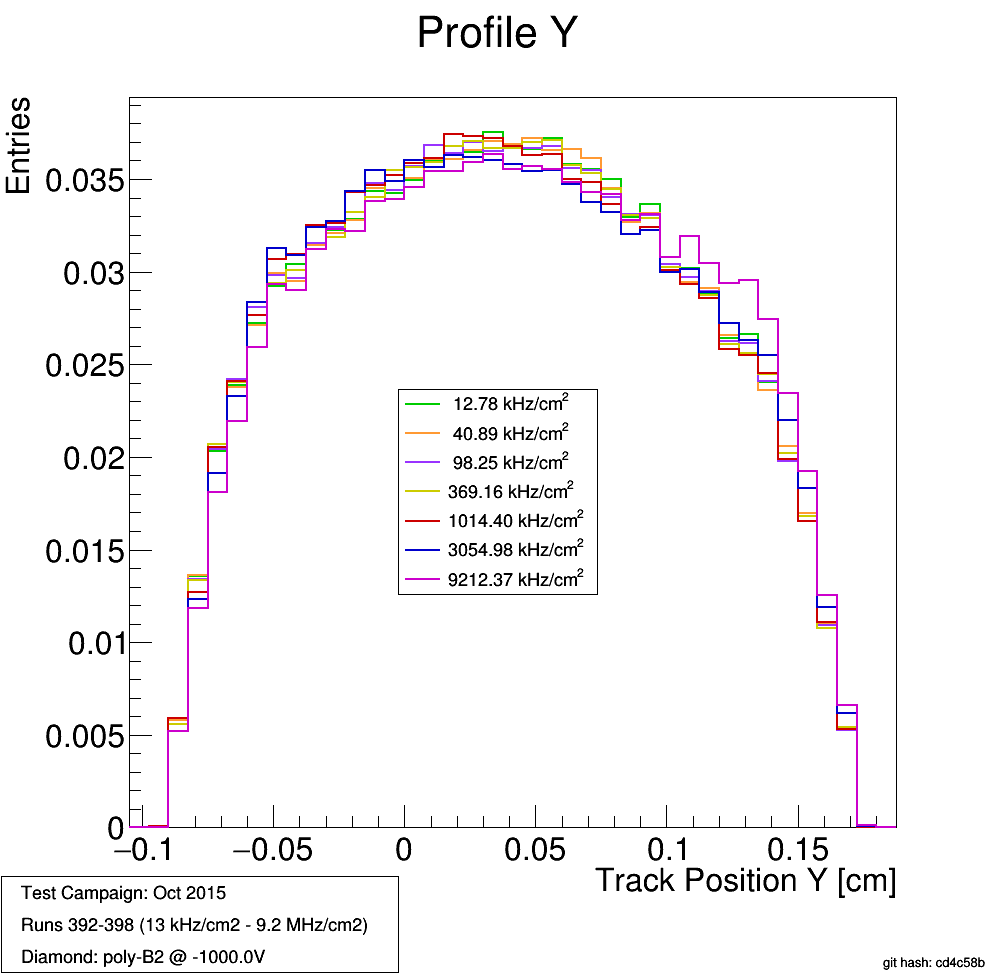
\includegraphics[width=5.5cm]{AllBeamProfilesY}
		\end{minipage}\no\s
	\end{center}
\end{frame}
% new frame ============================
\begin{frame}
	\begin{center}
		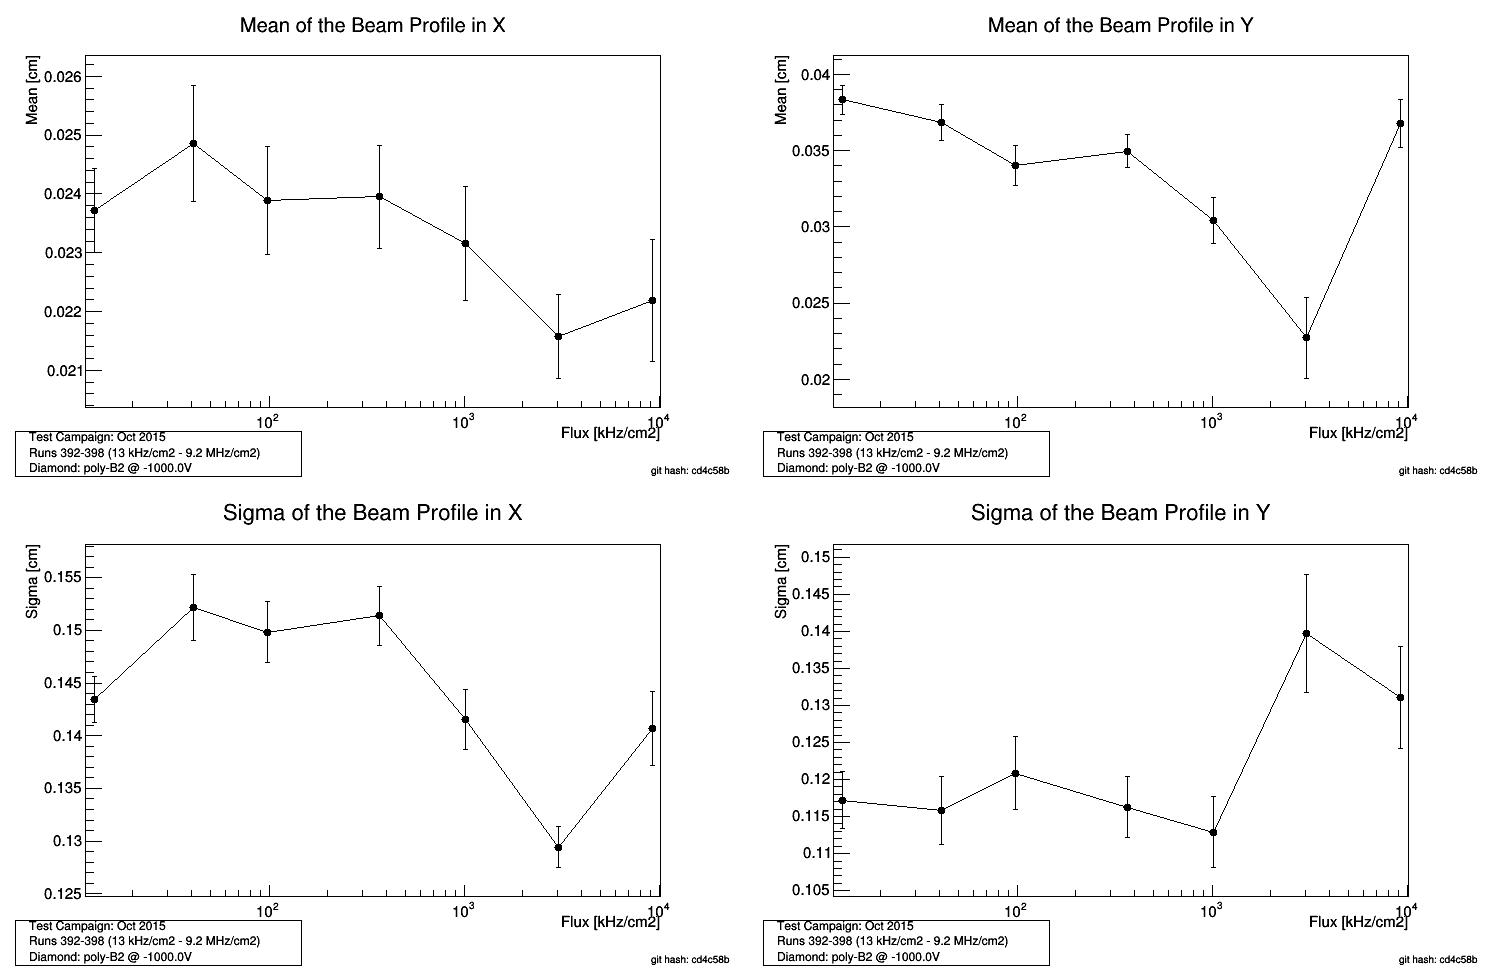
\includegraphics[width=10cm]{BeamProfileOverview}
	\end{center}
	\begin{itemize}
		\item $\chi^{2}\rightarrow1$
		\item x: 70\% range, y: 50\% range
	\end{itemize}
\end{frame}
% new frame ============================
\begin{frame}
	\begin{center}
		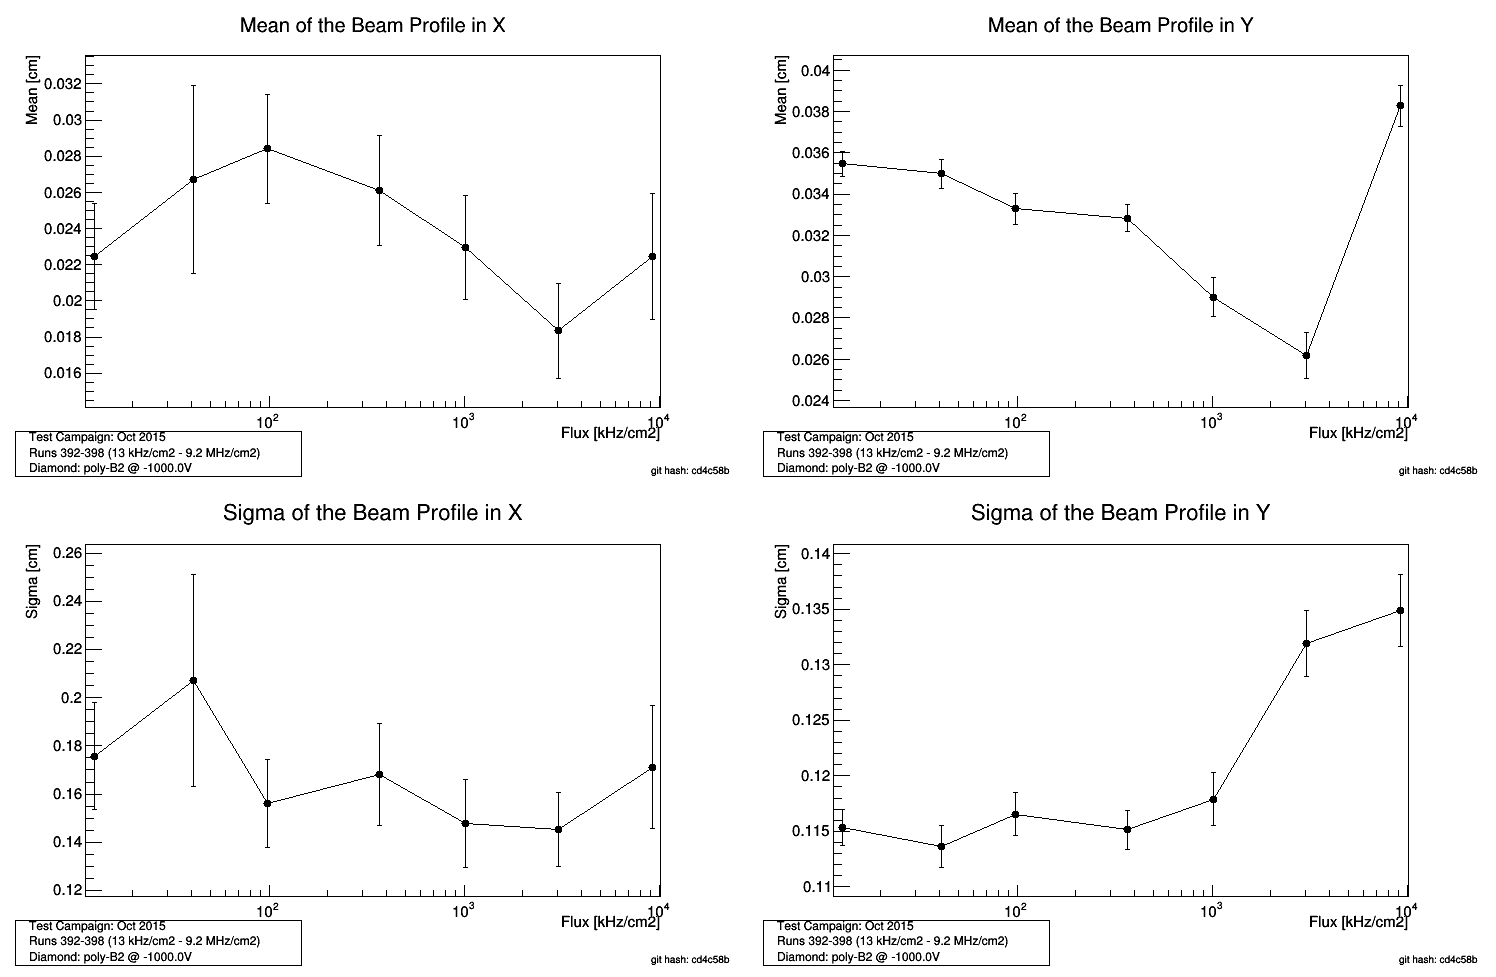
\includegraphics[width=10cm]{BeamProfileOverview2}
	\end{center}
	\begin{itemize}
		\item biggest sigmas
		\item x: 40\% range, y: 70\% range
	\end{itemize}
\end{frame}
% ====================================================================================
% \section{Pulser}
% % ============================
% \subsection{Pulser}
% \begin{frame}
% 	\begin{center}
% 		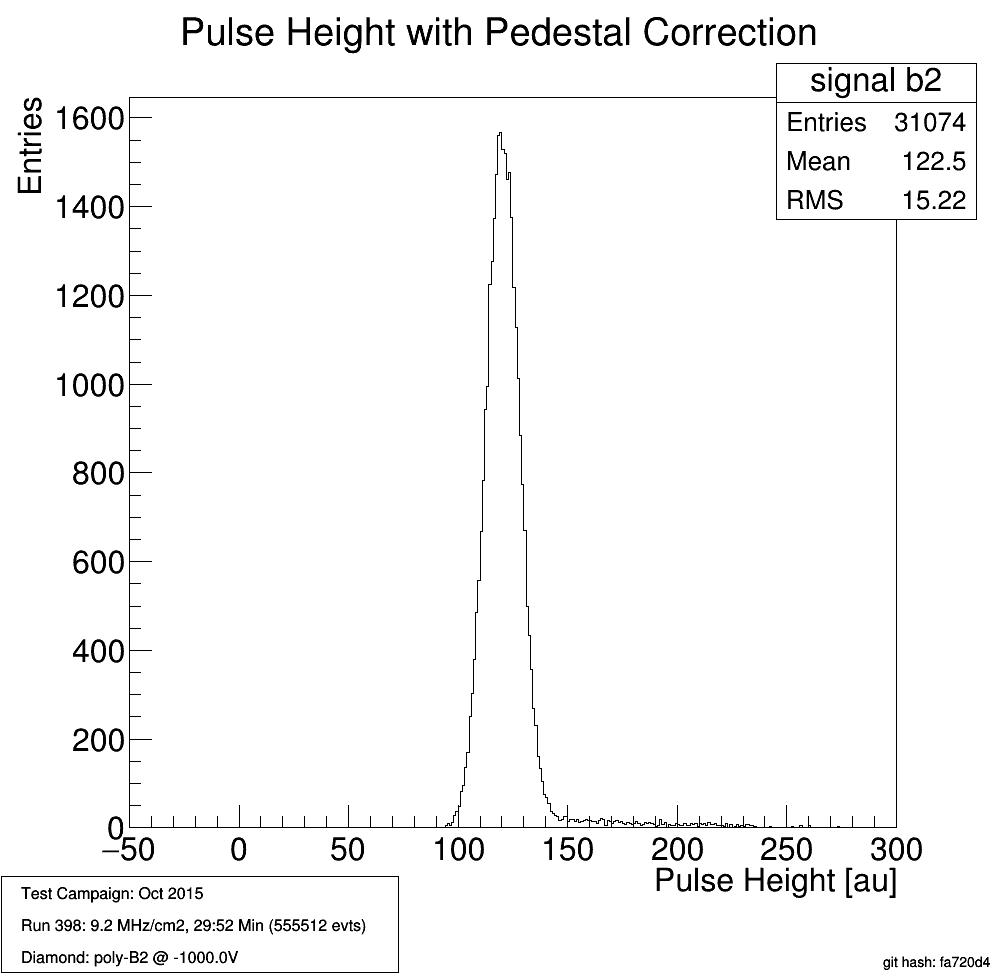
\includegraphics[width=5.5cm]{SignalDistribution}
% 	\end{center}
% \end{frame}
% % ============================
% \begin{frame}
% 	\begin{center}
% 		\begin{minipage}{5.5cm}
% 			\centering
% 			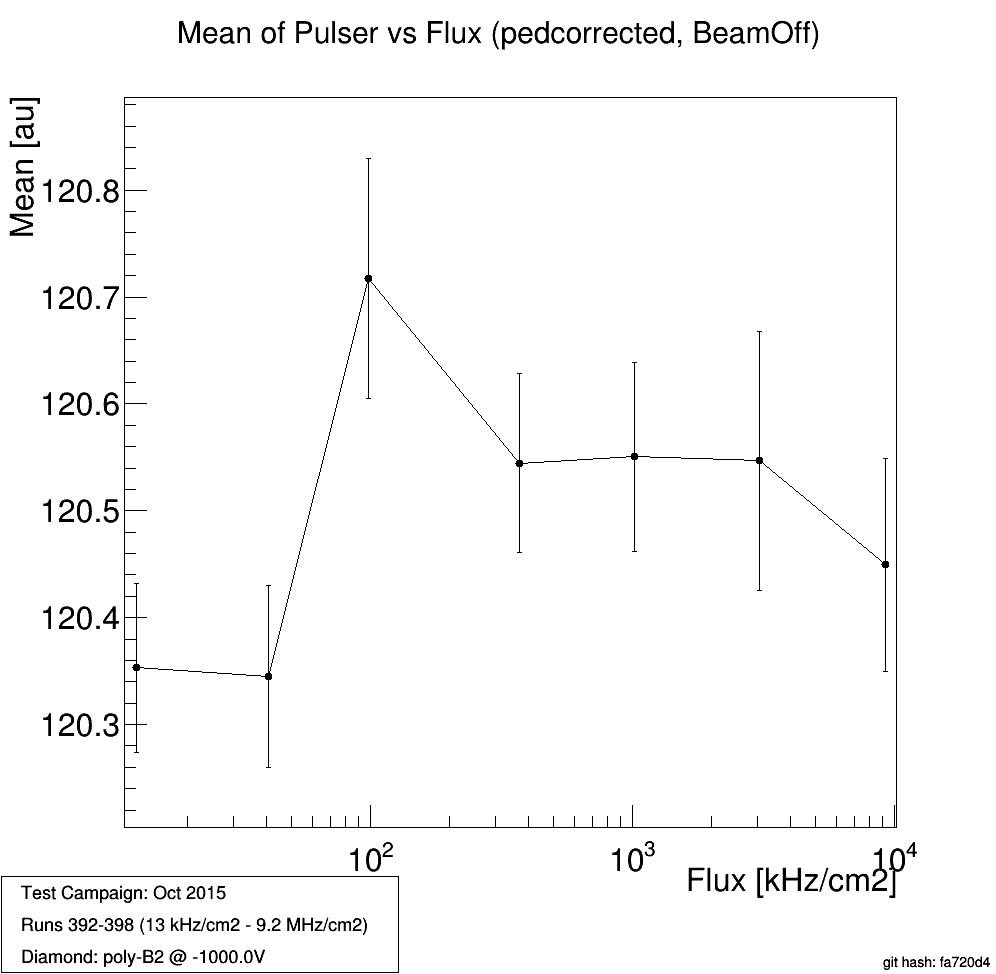
\includegraphics[width=5.5cm]{PulserMeanTrueTrue}
% 		\end{minipage}
% 		\hspace*{2pt}
% 		\begin{minipage}{5.5cm}
% 			\centering
% 			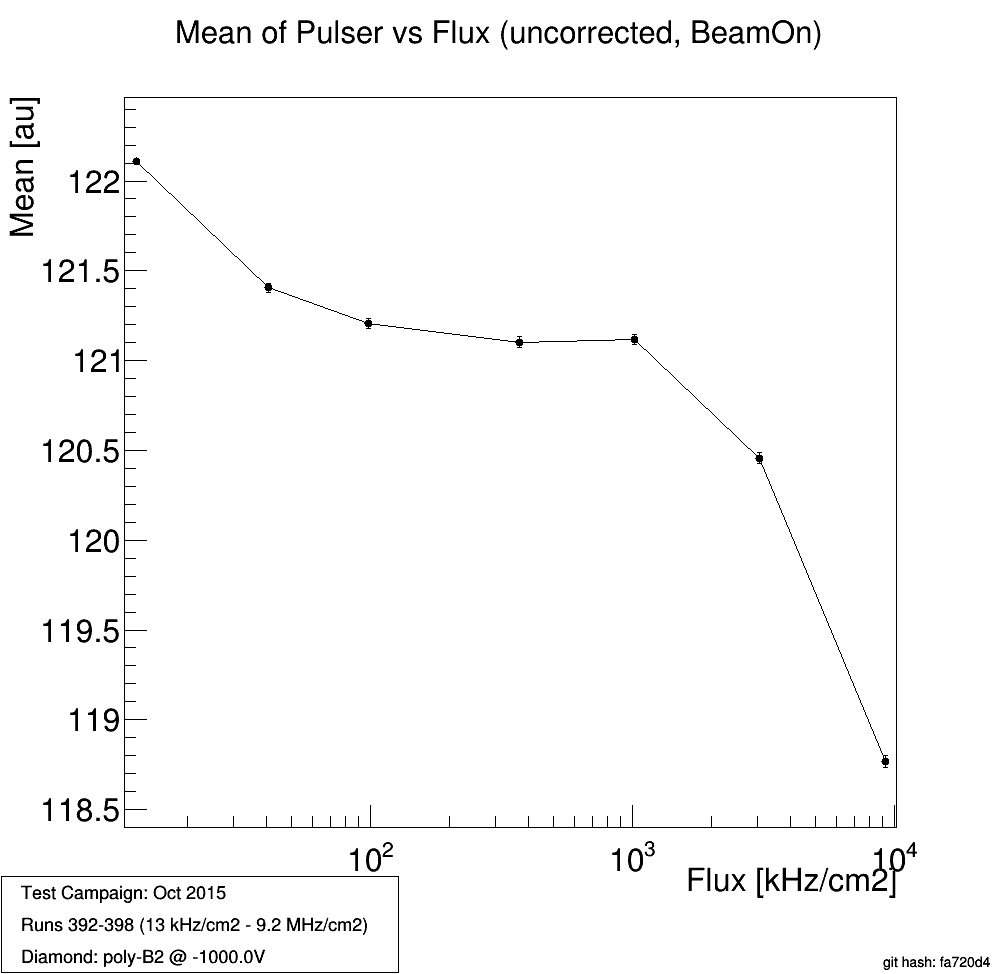
\includegraphics[width=5.5cm]{PulserMeanFalseFalse}
% 		\end{minipage}\no\s
% 	\end{center}
% \end{frame}
% % ============================
% \begin{frame}
% 	\begin{center}
% 		\begin{minipage}{5.5cm}
% 			\centering
% 			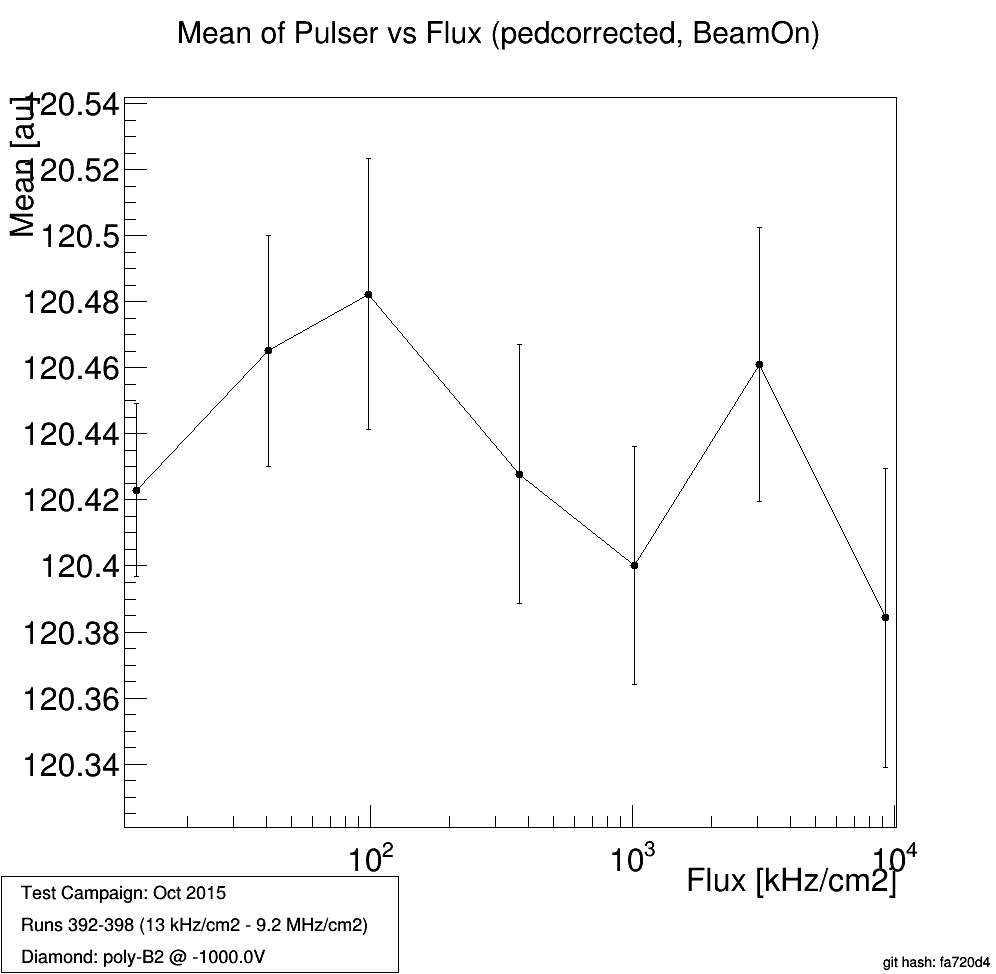
\includegraphics[width=5.5cm]{PulserMeanTrueFalse}
% 		\end{minipage}
% 		\hspace*{2pt}
% 		\begin{minipage}{5.5cm}
% 			\centering
% 			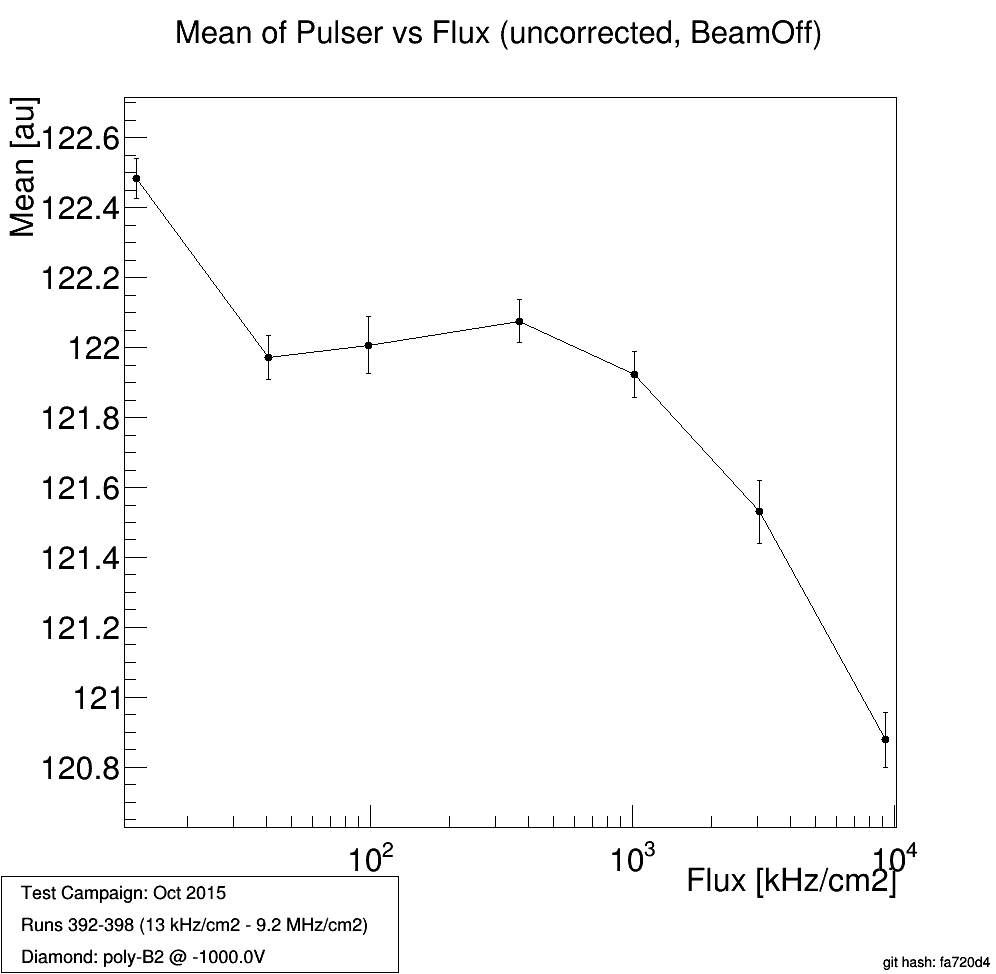
\includegraphics[width=5.5cm]{PulserMeanFalseTrue}
% 		\end{minipage}\no\s
% 	\end{center}
% \end{frame}
% % ============================
% \begin{frame}
% 	\begin{center}
% 		\begin{minipage}{5.5cm}
% 			\centering
% 			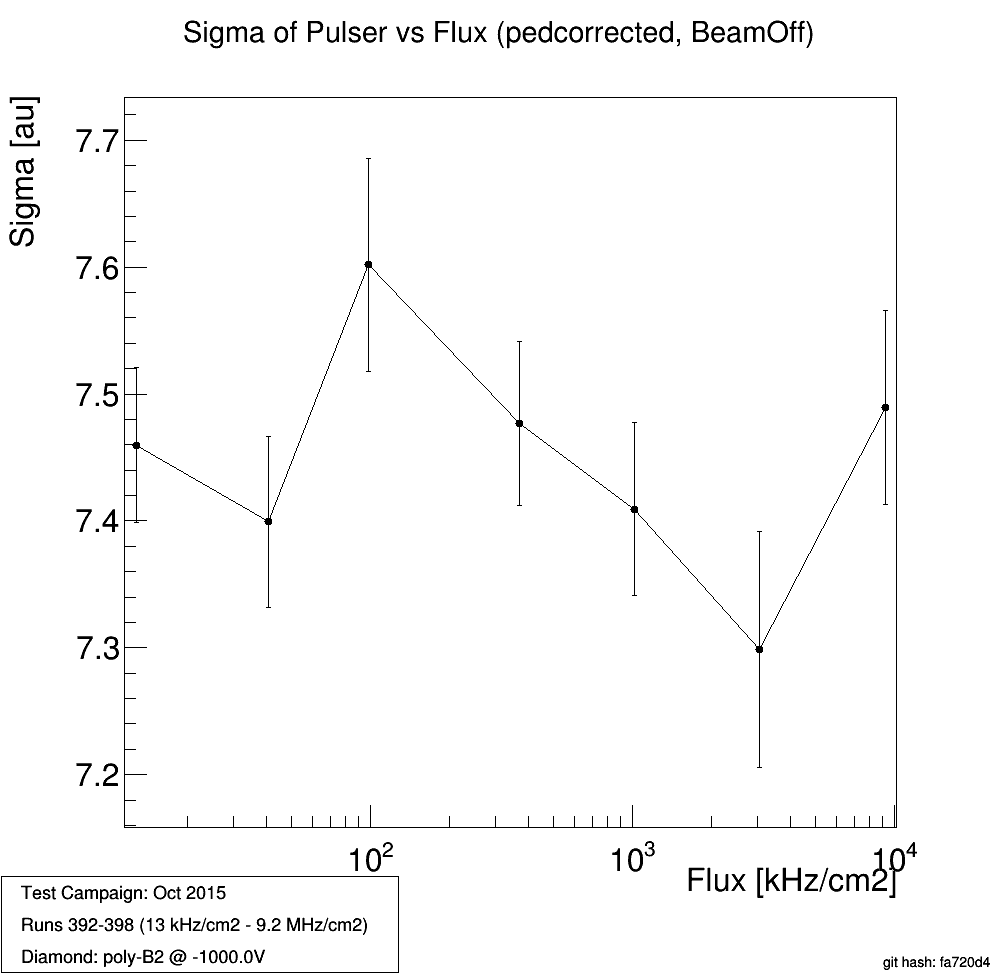
\includegraphics[width=5.5cm]{PulserSigmaTrueTrue}
% 		\end{minipage}
% 		\hspace*{2pt}
% 		\begin{minipage}{5.5cm}
% 			\centering
% 			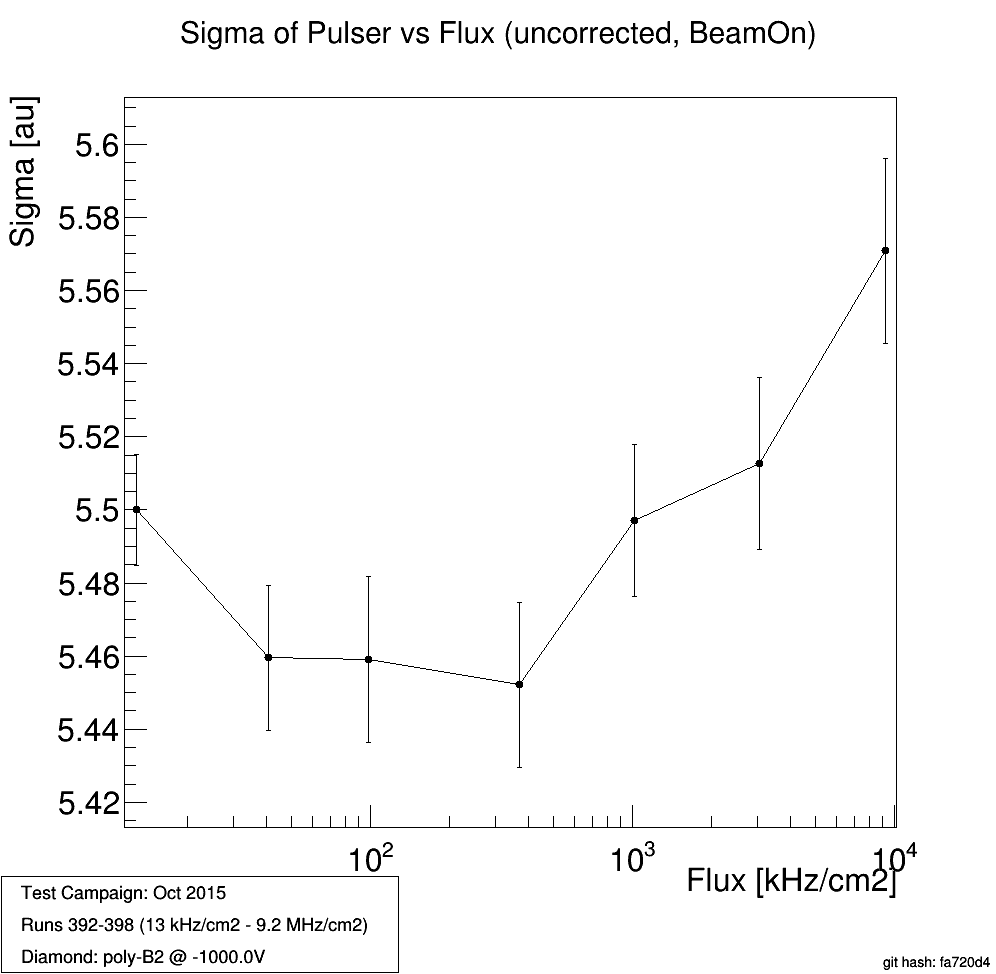
\includegraphics[width=5.5cm]{PulserSigmaFalseFalse}
% 		\end{minipage}\no\s
% 	\end{center}
% \end{frame}
% % ============================
% \begin{frame}
% 	\begin{center}
% 		\begin{minipage}{5.5cm}
% 			\centering
% 			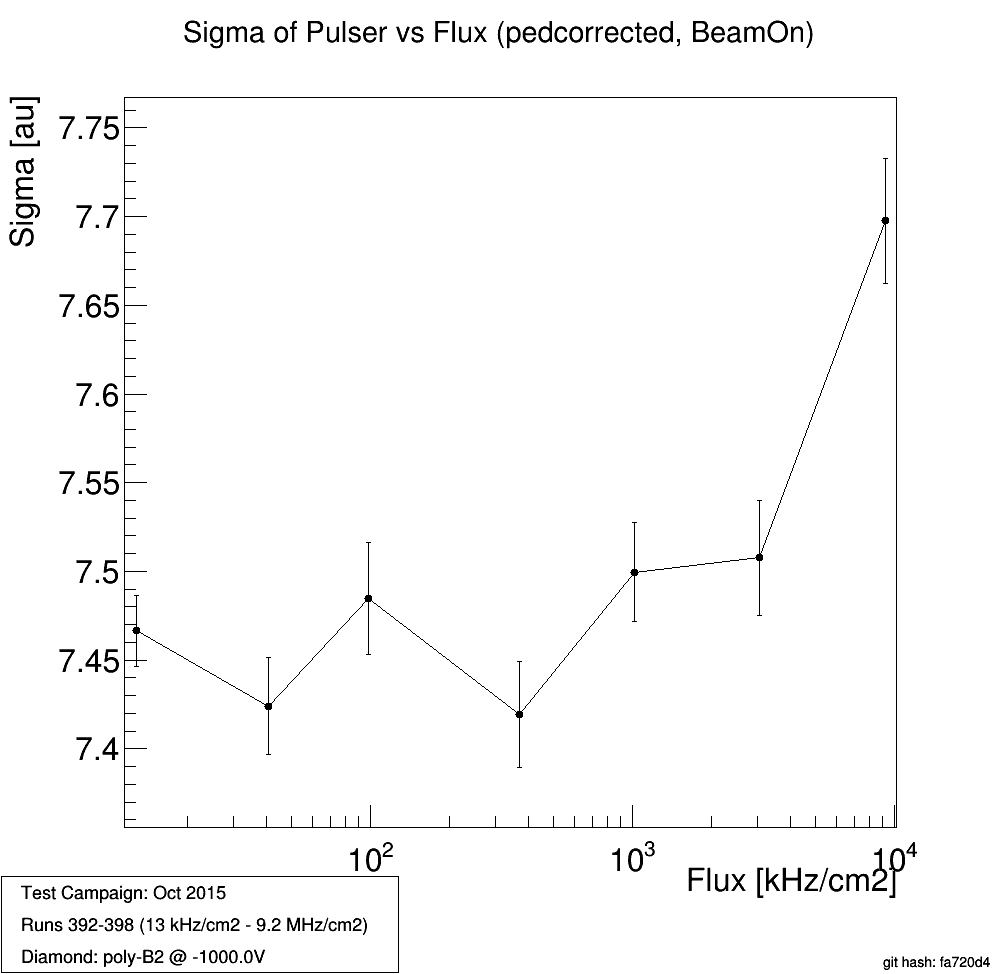
\includegraphics[width=5.5cm]{PulserSigmaTrueFalse}
% 		\end{minipage}
% 		\hspace*{2pt}
% 		\begin{minipage}{5.5cm}
% 			\centering
% 			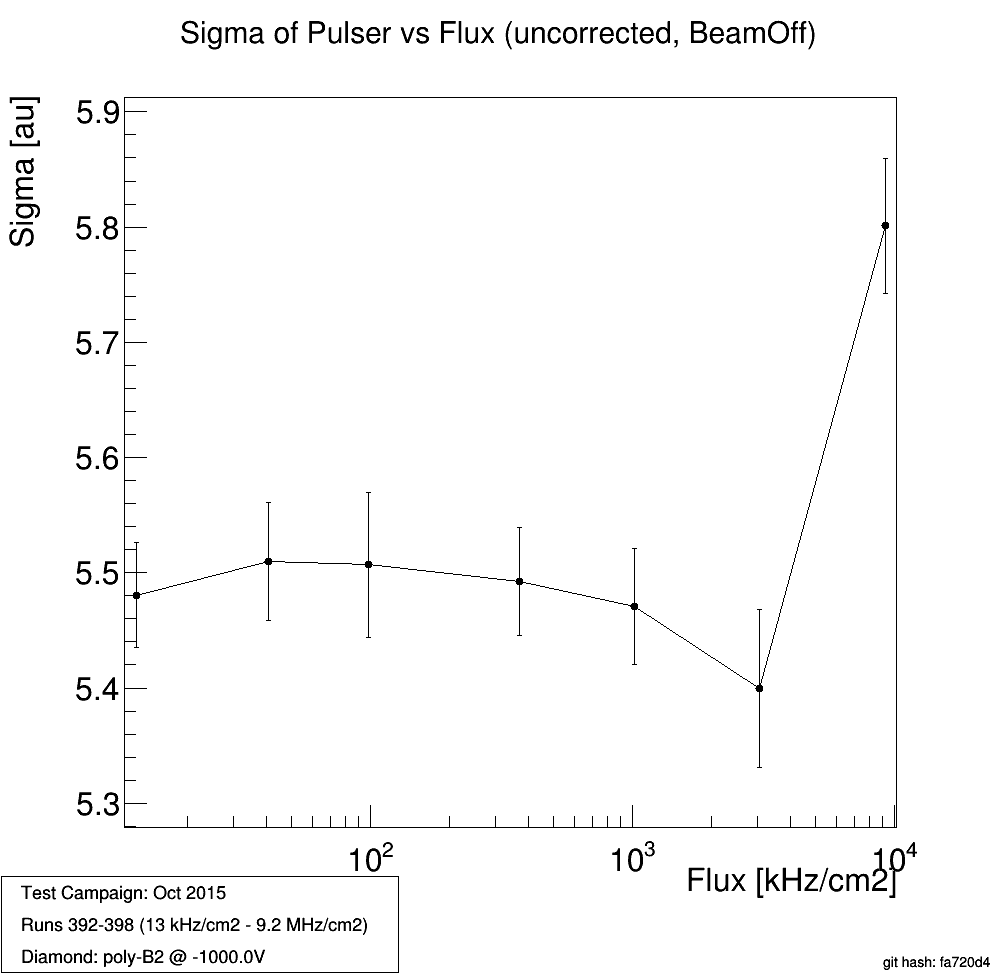
\includegraphics[width=5.5cm]{PulserSigmaFalseTrue}
% 		\end{minipage}\no\s
% 	\end{center}
% \end{frame}
% ============================
% ====================================================================================
\section{Pulse height distribution}
\subsection{Pulse height distribution}
\begin{frame}
	\begin{center}
		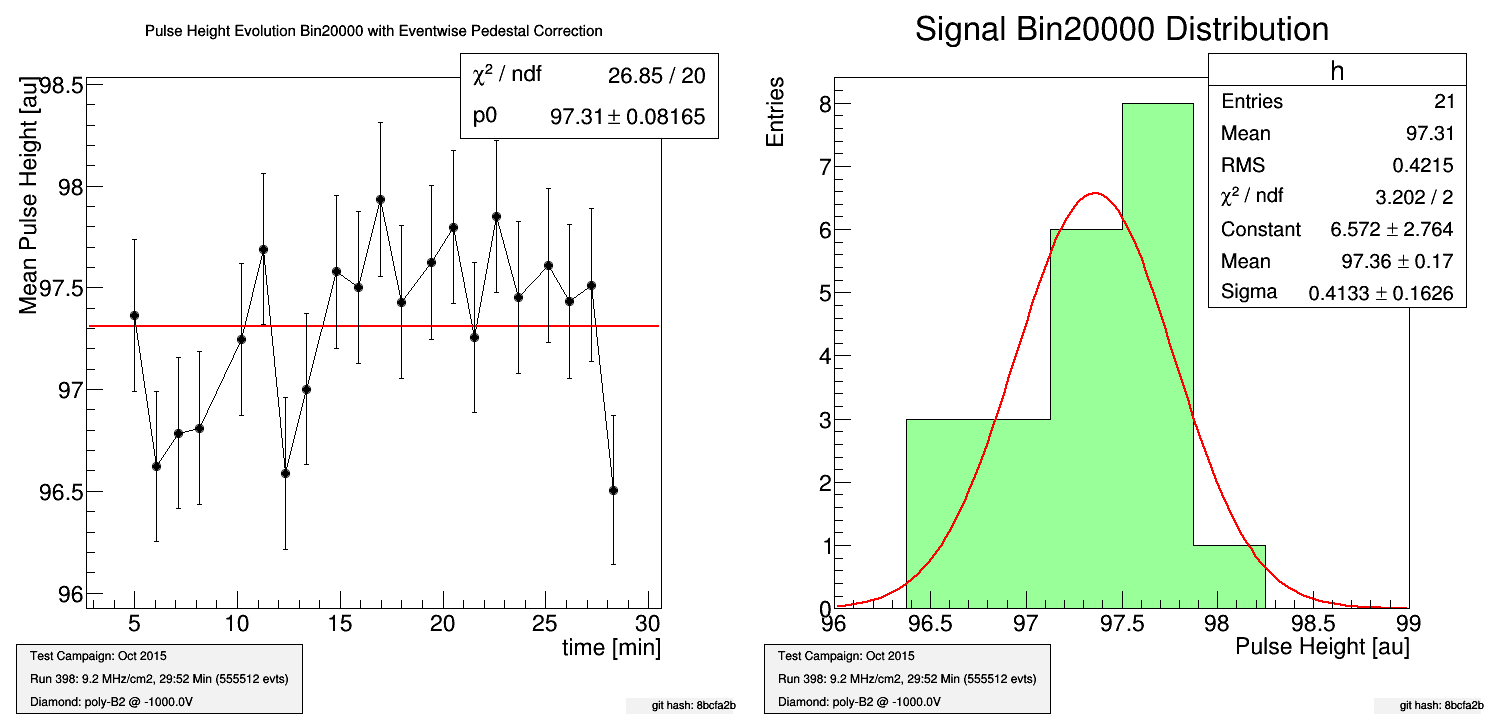
\includegraphics[width=8cm]{PHEvolutionOverview20000}
	\end{center}
	\begin{center}
		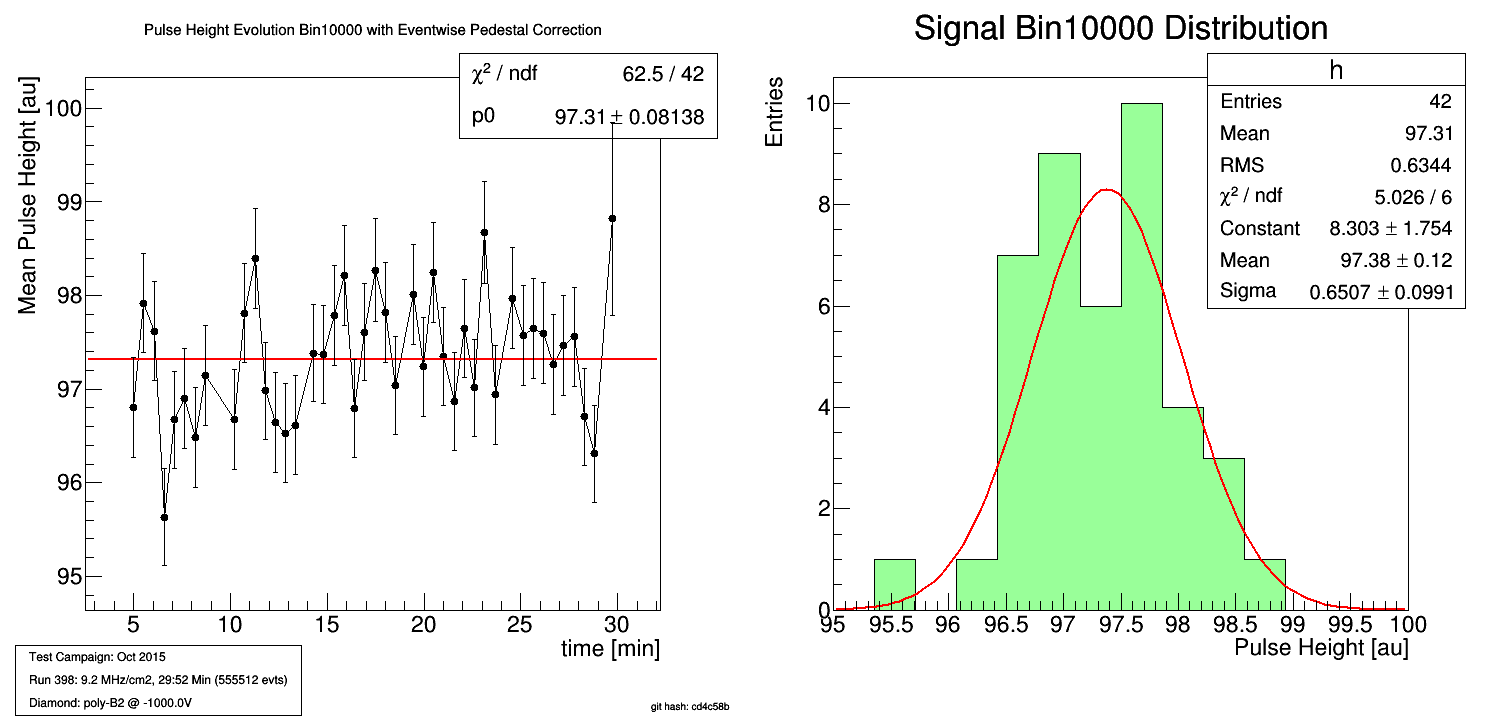
\includegraphics[width=8cm]{PHEvolutionOverview10000}
	\end{center}
\end{frame}
% ============================
\begin{frame}
	\begin{center}
		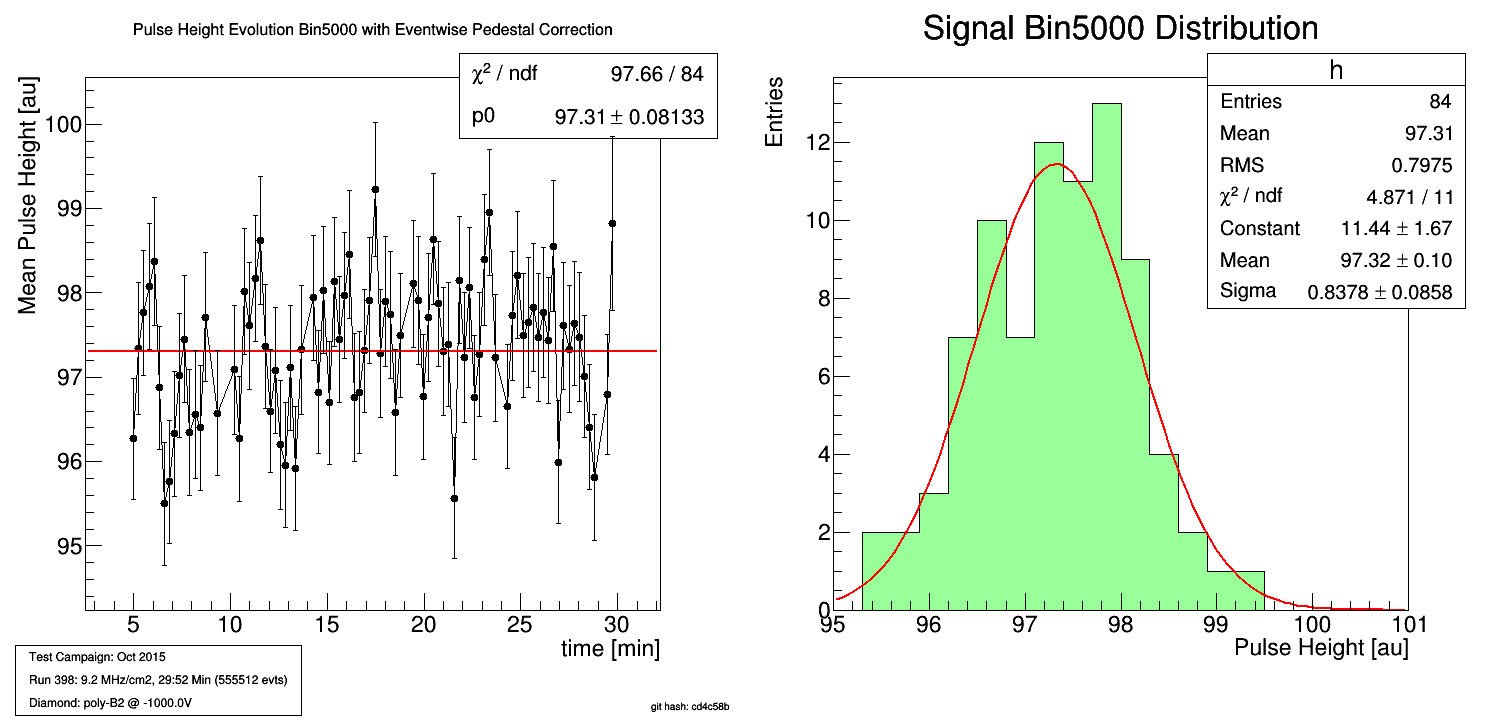
\includegraphics[width=8cm]{PHEvolutionOverview5000}
	\end{center}
	\begin{center}
		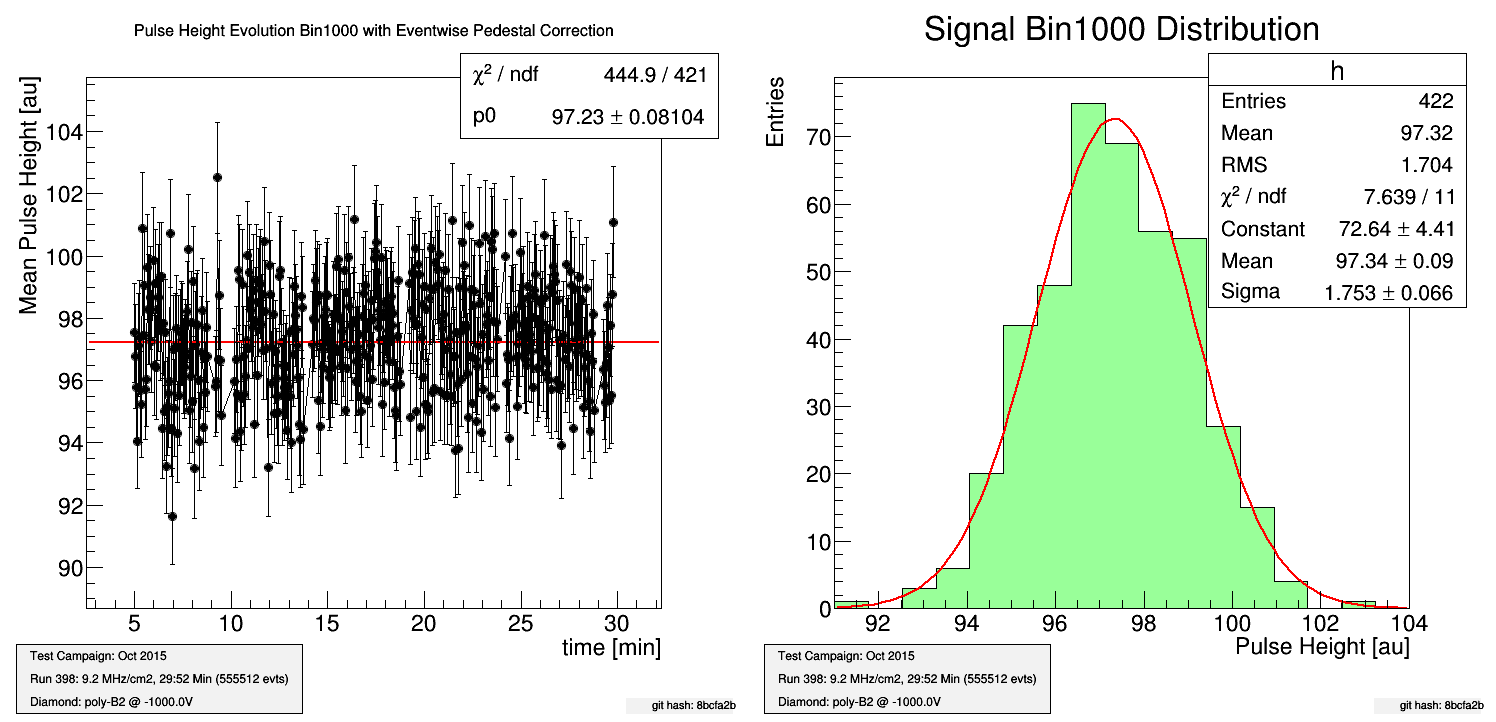
\includegraphics[width=8cm]{PHEvolutionOverview1000}
	\end{center}
\end{frame}
% ============================
\begin{frame}
	\begin{center}
		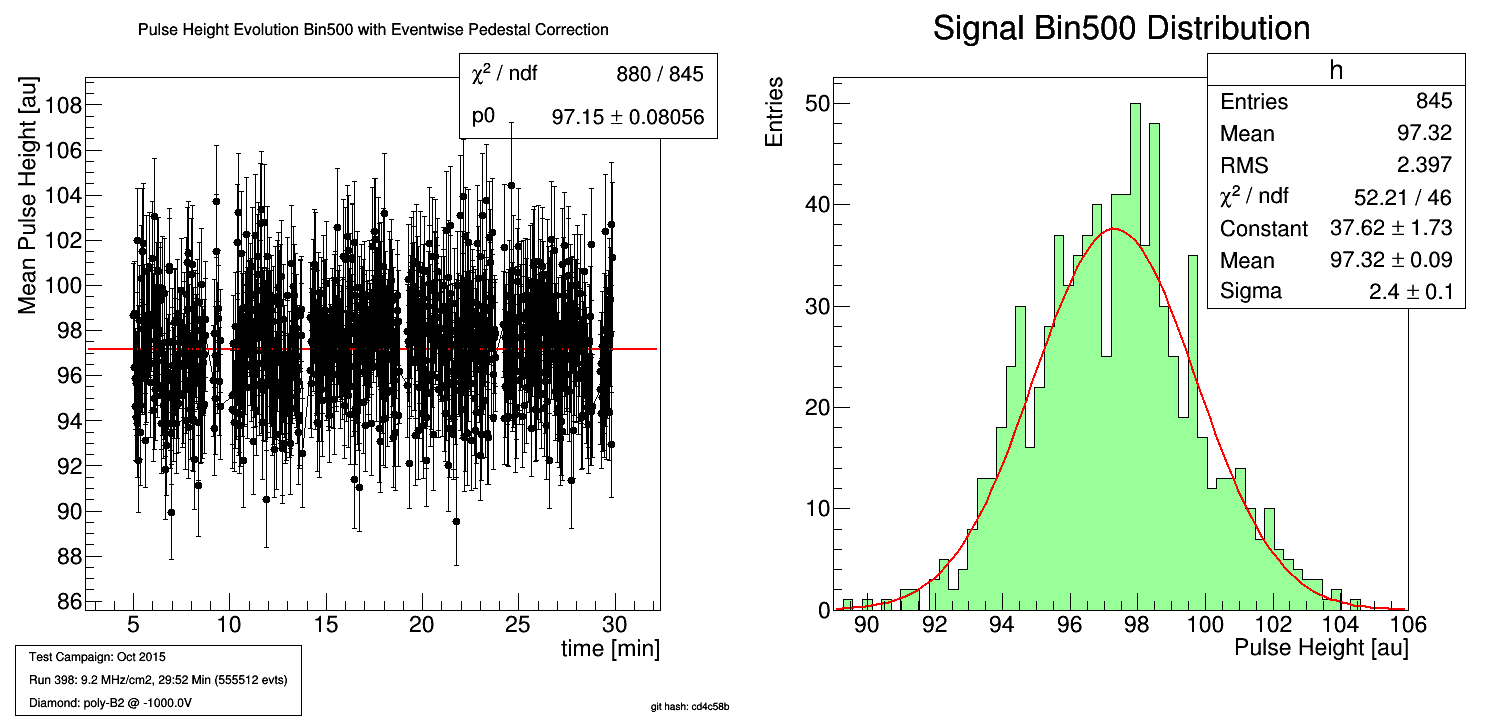
\includegraphics[width=8cm]{PHEvolutionOverview500}
	\end{center}
	\begin{center}
		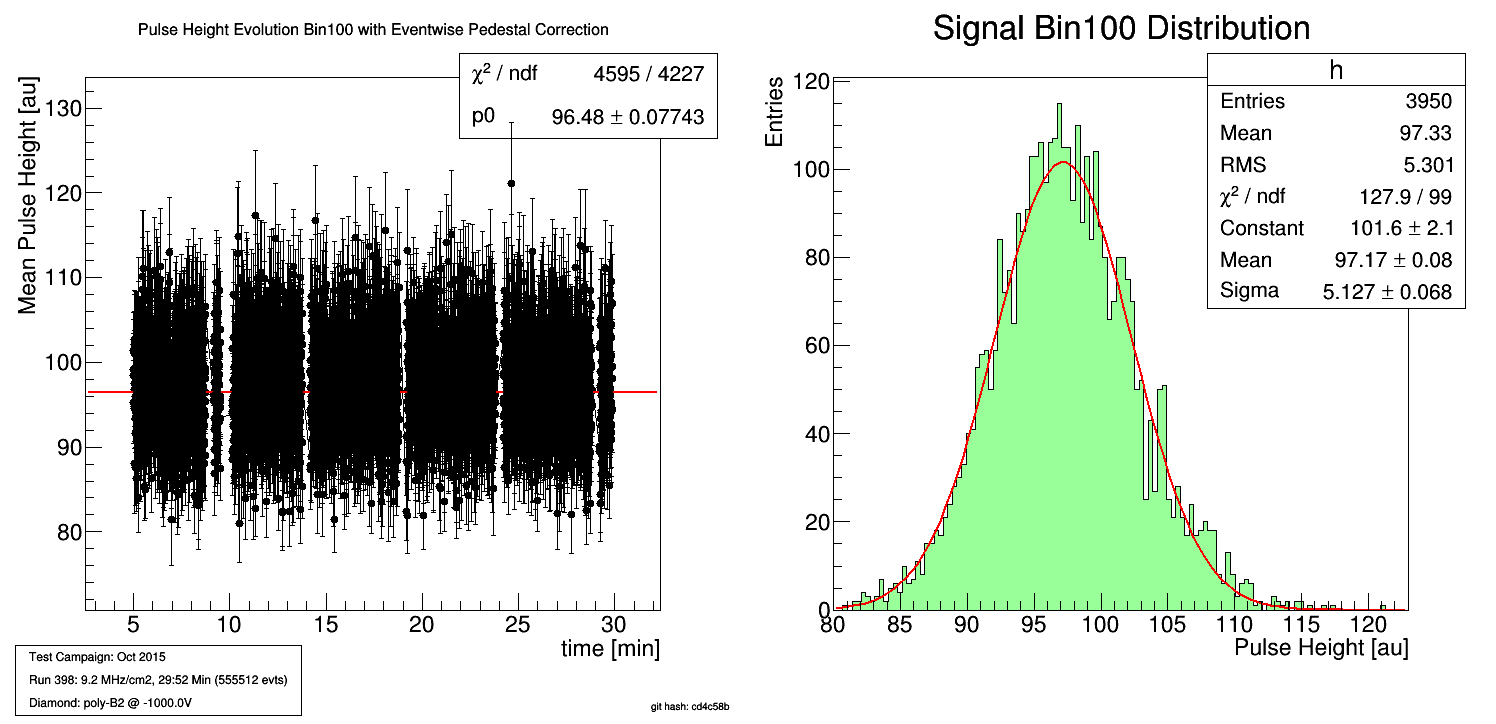
\includegraphics[width=8cm]{PHEvolutionOverview100}
	\end{center}
\end{frame}
% ============================
% DOCUMENT END
\end{document}

